% Paper 3 -- skeleton written at the setup of Ralph loop0015 (2026-11-05).
%
% Build: `make` in this directory (latexmk -pdf); `make check` fails on any
% undefined reference or citation. House setup copied from paper1/latex/main.tex
% (article class, Palatino, natbib plainnat, Appendix A of Lean names).
%
% THE TITLE IS FIXED BY THE OWNER AND MUST STAY VERBATIM, INCLUDING THE ELLIPSIS
% AND THE FINAL PERIOD. The plain string is:
%   Exponential time hypothesis is false... but the verified algorithm is slower than trying all 2^n assignments at every practical size.
% In \title below `$2^n$` and `\ldots` are its only LaTeX; the pdftitle carries
% the plain string. The gate (Ralph_Loops/loop0015/gate.py) checks it. Questions
% about the wording go to ../ETH_AMBIGUOUS.MD, never into the title.
\documentclass[11pt,letterpaper]{article}

\usepackage[T1]{fontenc}
\usepackage[utf8]{inputenc}
\usepackage[sc]{mathpazo}
\linespread{1.05}
\usepackage{courier}
\usepackage[protrusion=true,expansion=false]{microtype}
\usepackage[margin=1in]{geometry}
\usepackage{amsmath,amssymb,amsthm}
\usepackage{graphicx}
\usepackage{booktabs}
\usepackage{array}
\usepackage{tabularx}
\usepackage{longtable}
\usepackage{caption}
\usepackage{float}
\usepackage[section]{placeins}
\usepackage{xcolor}
\usepackage[hyphens]{url}
\usepackage[title,titletoc]{appendix}
\usepackage[authoryear,round]{natbib}
\usepackage[colorlinks=true,linkcolor=blue!50!black,citecolor=blue!50!black,urlcolor=blue!50!black]{hyperref}
\hypersetup{pdftitle={Exponential time hypothesis is false... but the verified algorithm is slower than trying all 2\string^n assignments at every practical size.}}

\graphicspath{{figures/}}
\numberwithin{figure}{section}
\numberwithin{table}{section}
\captionsetup{font=small,labelfont=bf}
\bibliographystyle{plainnat}

% Lean names live in Appendix A (secA_appendix_lean.tex), one entry per
% result, as in paper 1: \leanentry{key}{result} opens a row, \leannames{a, b}
% prints the names, and the text cites an entry with \leanref{key}.
\makeatletter
\g@addto@macro{\UrlBreaks}{\do\_\do\.}
\newcommand{\leannames}[1]{\def\lean@sep{}\@for\lean@n:=#1\do{\lean@sep\expandafter\path\expandafter{\lean@n}\def\lean@sep{, }}}
\makeatother
\newcounter{leanentry}
\renewcommand{\theleanentry}{A.\arabic{leanentry}}
\newcommand{\leanentry}[2]{\leavevmode\refstepcounter{leanentry}\label{lean:#1}\theleanentry & #2 &}
\newcommand{\leangroup}[1]{\multicolumn{3}{@{}l}{\emph{#1}}\\}
\newcommand{\leanref}[1]{(Appendix~\ref{app:lean}, \ref{lean:#1})}

\theoremstyle{plain}
\newtheorem{theorem}{Theorem}[section]
\newtheorem{lemma}[theorem]{Lemma}
\newtheorem{proposition}[theorem]{Proposition}
\newtheorem{corollary}[theorem]{Corollary}
\theoremstyle{definition}
\newtheorem{definition}[theorem]{Definition}
\theoremstyle{remark}
\newtheorem*{remark}{Remark}

% The verified exponent, rho(n) = n (ln ln(n+16))^2 / sqrt(ln(n+16)), and the
% comparator's names, used throughout.
\newcommand{\rhon}{\rho(n)}
\newcommand{\runtimeScale}{\texttt{runtimeScale}}
\newcommand{\SubexpCount}{\texttt{SubexpCount}}
% Paths in the repository and in the clone; a placeholder box for text an item
% still owes, as in paper 1.
\newcommand{\repofile}[1]{\path{#1}}
\newcommand{\clonefile}[1]{\path{#1}}
\newcommand{\placeholder}[1]{\par\noindent\fbox{\parbox{\dimexpr\linewidth-2\fboxsep-2\fboxrule}{\textbf{Placeholder.} #1}}\par}

% Title: fixed by the owner, verbatim (see the comment at the top).
\title{Exponential time hypothesis is false\ldots{} but the verified algorithm is slower than trying all $2^n$ assignments at every practical size.}
% Author line resolved by the owner on 2026-11-05 (ETH_AMBIGUOUS.MD, S1): Alex Linhares,
% Argo Lab AGI, on leave from the Getulio Vargas Foundation, ORCID as in paper 1.
% The AI contribution is disclosed in the acknowledgements in paper 1's form.
\author{Alex Linhares\\{\small Argo Lab AGI; on leave from the Getulio Vargas Foundation}\\{\small \href{mailto:alex@argolab.org}{alex@argolab.org} \quad ORCID \href{https://orcid.org/0000-0002-4227-6879}{0000-0002-4227-6879}}}
\date{\today}

\begin{document}
\maketitle

\begin{abstract}
\noindent
\placeholder{Item 09 writes the abstract (under 200 words; no number without a
section that regenerates it). The title's sentence made precise: what is
verified is a guarantee with existential constants and the exponent
$n(\log\log n)^2/\sqrt{\log n}$, whose factor exceeds $1$ for every
$50 \le n < e^{5504}$, so the verified guarantee is weaker than the trivial
$2^n \cdot \mathrm{poly}$ guarantee at every practical size; the machine's
running time is unknown because the constants are never computed; the
manuscript's sharper exponents are unverified; the statement does refute
ETH; the audit found no flaw.}
\end{abstract}

% Introduction -- drafted by loop0015 item 09 (2026-11-05), under the owner's
% plain-English rule of 2026-11-05 05:30: no formula beyond 2^n in this
% section, every term of art glossed in one clause on first use, every
% number with the section that regenerates it. The title's four clauses are
% made precise in the first paragraph; the symbols (the exponent, the
% constants) are introduced in Section 2 and used from there on. A blind
% reader's pass (one subagent, 2026-11-05) moved the glossary ahead of the
% summary and shortened the long sentences.
\section{Introduction}
\label{sec:intro}

In late October 2026, OpenAI's collection of machine-checked mathematics
added a result dated 25 October 2026 that it calls family 378,
\emph{The Exponential Time Hypothesis is False}
\citep{OAI:The-Exponential-Time-Hypothesis-is-False-October-25-2026}.
The Exponential Time Hypothesis, ETH, is a conjecture from 2001
\citep{ImpagliazzoPaturi2001}. It says that deciding whether a formula
with three variables per clause can be satisfied needs time that grows
exponentially in the number of variables. The result comes with a
67-page manuscript and a proof checked by the Lean proof assistant, a
program that verifies every step of a proof and rejects a proof with a
gap. The verified theorem does refute the hypothesis. The title of this
paper says what else is true of it. Its sentence has four clauses.
First, what is verified is a \emph{guarantee}, not a running time. The
theorem says that a machine halts within a stated bound; it says
nothing about how long the machine actually takes on any input. Second,
the bound contains constants that the theorem only says \emph{exist}.
No value of any of them is computed anywhere. Where the proof does
write a value down, the constant in the exponent is at least 257
(Section~\ref{sec:statement}). Third, the \emph{exponent}, the quantity
that two is raised to in the bound, is a fixed function of the number
of variables. With every constant set to one, it is larger than the
number of variables at every size from 50 variables up to a number with
2,391 digits (Section~\ref{sec:statement}, Figure~\ref{fig:central}).
Over that whole range the verified bound is above $2^n$, the cost of
trying every one of the $2^n$ assignments of $n$ variables. So the
verified guarantee is weaker, at every practical size, than the
guarantee of the method everyone already has. Fourth, the manuscript
states two sharper exponents, which would make a different sentence.
Neither is in the Lean library, and the manuscript itself calls the
verified one ``the weaker exponent'' (Section~\ref{sec:beyond}).

This paper is a careful reading by people who checked, not a debunking.
We read the verified statement line by line. We inspected the proof's
source. We rebuilt the proof from source in isolation and re-checked it
with a second proof checker that shares no code with Lean's own. We
found no flaw: the statement means what the manuscript's verified form
says, and the proof rests on the three standard axioms, the assumptions
every ordinary Lean proof makes, and nothing else. Every sentence that
could read as ``wrong'' or ``overclaimed'' is replaced by what the Lean
statement and the manuscript actually say, with the file and line, or
the page and line, beside it. Nothing is quoted from memory. Every
number has a script that regenerates it, named where the number
appears.

\subsection{The words we use}
\label{sec:intro-words}

Each section glosses its own terms where they first appear, so that a
reader may enter anywhere. The ones the whole paper needs are these,
each in a sentence or two.
A \emph{formula} is a list of clauses, each clause an ``or'' of a few
variables or negated variables. A choice of true or false for every
variable \emph{satisfies} the formula when it makes every clause true.
A \emph{$k$-CNF} is a formula with at most $k$ variables per clause,
and $k$ is called the \emph{clause width}; 3-SAT is the problem of
deciding whether a 3-CNF can be satisfied.
\emph{Trying all $2^n$ assignments} is the method of checking every one
of the $2^n$ ways to set $n$ variables; its cost is the yardstick in the
title.
\emph{ETH} is the conjecture that 3-SAT needs time exponential in $n$.
\emph{SETH}, its strong form, says that as $k$ grows no algorithm for
$k$-SAT does much better than trying all assignments. Several variants
exist, and Section~\ref{sec:consequences} names each.
A \emph{guarantee} is a bound a theorem promises; a \emph{running time}
is what a clock measures; the two are compared only with their own
kind.
\emph{Lean} is the proof assistant. Its \emph{kernel} is the small core
that does the final checking, and ``verified'' in this paper always
means ``accepted by the kernel''. \emph{Mathlib} is Lean's community
library of mathematics.
The \emph{comparator} is OpenAI's checking tool. It takes a
\emph{challenge file}, which states a theorem with the proof left
blank, and a \emph{solution}, which proves it. It checks that both
state the same theorem and that the proof uses only the three standard
axioms.
\emph{nanoda} is a second, independent checker for Lean proofs, written
in another language. A \emph{replay} is a rebuild of a proof from
source on our own machine, inside a \emph{sandbox}, an isolated
environment that sees nothing else on the machine, at the \emph{pinned}
Lean version, the exact version the repository names.
A \emph{SAT solver} is the program a practitioner runs to decide a
formula, and a \emph{model counter} the one that counts its satisfying
assignments.

\subsection{What this paper does}
\label{sec:intro-summary}

In one paragraph. The verified statement (Section~\ref{sec:statement})
says that for each fixed clause width there exist a finite machine of
the textbook kind, a Turing machine with several tapes, and five
positive constants. On every formula of that width the machine halts
with the exact number of satisfying assignments written on a tape. It
does so within a bound: a constant, times a power of the input length,
times two raised to a constant times the exponent. The exponent is
written out in Section~\ref{sec:statement}. Its ratio to the number of
variables rises above one at 50, peaks at about 2.17 near a number with
24 digits, and falls back below one only past a number with 2,391
digits. The manuscript claims more than the statement
(Section~\ref{sec:beyond}): two sharper exponents; a bound on the size
of logic circuits that depends on one of them; and a chapter of proofs
by a technique of its own, tensor contraction. We tag every claim
verified, supported on paper by the verified statement, or paper-only.
We inspected the proof (Section~\ref{sec:proof}): all 3,091 source
files it depends on. They contain no axiom, no omitted proof, no step
that trusts a compiled program, and no patch to Mathlib, and the
statement they prove is the one the comparator posed. We replayed it
(Section~\ref{sec:replay}). The 3,091 files built from source in a
sandbox at the pinned Lean version in 33 minutes; the kernel reported
the three standard axioms; and nanoda re-checked 95,176 declarations,
the theorem and everything it depends on, with no error. We say what
follows (Section~\ref{sec:consequences}). The statement alone refutes
ETH, SETH, the gap form, the form for guessing (nondeterministic)
machines, the counting form, and the randomised forms of ETH, SETH and
the gap form. A lower bound that was proved \emph{from} one of them is
an ``if \ldots{} then'' whose ``if'' is now false: it derives nothing,
and the statement it concluded is not itself refuted. We say what it
changes for a practitioner (Section~\ref{sec:practitioner}): nothing on
any machine. We show that by timing an ordinary SAT solver and two model
counters on random formulas of up to 500 variables and drawing the two
guarantees beside the measurements. We restate the verified sentence in
our own Lean library under one name, with its axioms audited
(Section~\ref{sec:lean}). And we place the paper beside what the
collection, the hypotheses' authors, a published human audit, and the
two checking tools say about themselves (Section~\ref{sec:related}).

\subsection{What is claimed, and what is not}
\label{sec:intro-claims}

Claimed, each with the section that establishes it:
\begin{enumerate}
\item The verified statement is a running-time \emph{guarantee} with
  constants that exist and are never computed, for each fixed clause
  width, with no lower limit on the number of variables
  (Section~\ref{sec:statement}).
\item With every constant set to one, the verified exponent exceeds the
  number of variables at every size from 50 up to a number with 2,391
  digits, so the verified bound is above $2^n$ there. The true constants
  are unknown and at least 257 in the proof on record, so with them the
  bound is higher still (Section~\ref{sec:statement}).
\item The manuscript's two sharper exponents, and the circuit bound that
  rests on one of them, are not in the Lean library
  (Section~\ref{sec:beyond}).
\item The proof's source shows none of the known ways of weakening a
  verified proof, and its statement is the challenge's
  (Section~\ref{sec:proof}). It builds from source at the pinned
  version with the three standard axioms, and a second checker agrees
  (Section~\ref{sec:replay}).
\item The verified statement refutes ETH, SETH, their gap, guessing and
  counting forms, and the randomised forms of ETH, SETH and the gap
  form, by the parts of the statement named in each case. A lower bound
  derived from any of them loses its premise and nothing more
  (Section~\ref{sec:consequences}).
\item On random formulas, the solvers a practitioner has are many
  orders of magnitude below $2^n$ at every size measured, and the
  verified guarantee is above $2^n$ from 50 variables on. The verified
  result changes nothing that runs (Section~\ref{sec:practitioner}).
\end{enumerate}
Not claimed:
\begin{enumerate}
\item No running time of the verified machine, in either direction. No
  implementation of it exists; the title compares two guarantees.
\item No flaw in the statement, the proof, the Lean kernel, Mathlib, or
  the collection's checking tool. We found none and assert none.
\item No value of any constant beyond what the proof writes down, and
  nothing about what a different proof of the same statement could
  achieve.
\item No judgement on the manuscript's paper-only proofs, which were
  located and quoted, not read for correctness.
\item No refutation of any lower bound's conclusion, for any problem,
  and nothing about any specific problem's complexity beyond what the
  manuscript's own remarks state.
\item Nothing about any problem outside satisfiability. This paper is
  about the limitation of the ETH refutation and nothing else.
\end{enumerate}

\subsection{How the paper is organised}
\label{sec:intro-organisation}

Section~\ref{sec:statement} reads the statement.
Section~\ref{sec:beyond} draws the line between it and the manuscript.
Sections~\ref{sec:proof} and \ref{sec:replay} inspect and replay the
proof. Section~\ref{sec:consequences} says what follows.
Section~\ref{sec:practitioner} is for the practitioner.
Section~\ref{sec:lean} is our own Lean. Section~\ref{sec:related} is
related work. Section~\ref{sec:conclusion} concludes and lists the
questions this reading left for its author to decide. Every section
ends with a list headed ``what this does not claim''.
Appendix~\ref{app:lean} lists every Lean name the paper cites.
Appendix~\ref{app:tech} holds the technical detail behind the plain
text of the body: the definitions with their line numbers, the theorem
with its quantifiers, the spine of the proof. The OpenAI repository is
read throughout at one commit, \texttt{4eaee875}, as untrusted data:
with text tools only, never built or run in place. The one build is the
sandboxed replay.

\subsection{What this does not claim}
\label{sec:intro-not}

\begin{itemize}
\item \textbf{Nothing beyond the sections it summarises.} Every
  sentence of this introduction is a sentence of a later section said
  shorter; where the two differ, the later section, with its file and
  line, is the one that counts.
\item \textbf{Nothing about the result's importance.} Whether the
  refutation matters is not a question this paper asks; what the
  verified statement says, and at what sizes, is.
\item \textbf{No prior-art claim.} ``We found no earlier statement'' of
  the title's observation is bounded to the six texts
  Section~\ref{sec:related} names; the literature at large was not
  searched.
\end{itemize}

% The verified statement, read exactly -- drafted by loop0015 item 02 (2026-11-05),
% rewritten in plain English by item 08x (2026-11-05, owner's rule of 05:30).
% Every line number of the comparator file is at commit 4eaee875 of the clone
% (~/dev/untrusted/openai-math, read with cat/sed -n only); every manuscript quote
% gives the page of paper.pdf and the line of reports/scratch/eth_audit/paper.txt.
% Every number of this section: python3 -I paper3/scripts/runtime_scale.py
% (the rho(n)/n table and the crossings) and python3 -I
% reports/scratch/eth_audit/check_encoding.py (the encoding lengths).
% The definition-by-definition reading and the theorem with its quantifiers
% are in Appendix B (secB_appendix_technical.tex), cited from here.
\section{The verified statement, read exactly}
\label{sec:statement}
\begingroup\sloppy

\subsection{What we are reading, and the words we need}
\label{sec:statement-words}

OpenAI's collection \citep{OAI:The-Exponential-Time-Hypothesis-is-False-October-25-2026}
holds, for the result it calls family 378, one machine-checked theorem.
It is named \path{exact_count_and_sat}. It is stated in the family's
challenge file, which is 220 lines long:
\clonefile{lean/ComparatorChallenges/SubexponentialSAT.lean} at commit
\texttt{4eaee875} of the collection. This section reads that
file and says what the theorem asserts and what it does not. Line
numbers are those of the file. We quote nothing from memory.

A few words first, each in one sentence.
\emph{Lean} is a proof assistant: a program that checks every step of a
proof and refuses a proof with a gap.
The \emph{kernel} is the small core of Lean that does the final
checking; when we say a statement is verified, we mean the kernel
accepted a proof of it.
A \emph{formula} here is a Boolean formula in conjunctive normal form: a
list of \emph{clauses}, each clause an ``or'' of a few variables or
negated variables, and the whole formula true when every clause is
true. A \emph{$k$-CNF} is such a formula whose clauses have at most $k$
variables each; 3-SAT is the problem of deciding whether a 3-CNF can be
made true.
A \emph{satisfying assignment} is a choice of true or false for every
variable that makes the formula true; with $n$ variables there are
$2^n$ assignments to try, and \emph{trying all $2^n$ assignments} is the
method the title names.
The \emph{comparator} is OpenAI's checking tool. It takes a
\emph{challenge file}, which states a theorem and leaves the proof blank,
and a \emph{solution}, which proves it, and checks that the two state
the same theorem and that the proof uses only three standard axioms. An axiom is a statement accepted without proof; the three standard ones are the ones every ordinary mathematical proof in Lean uses.
The file we read is the challenge file. It carries the statement with
the placeholder \texttt{sorry} where the proof would go (line 218). The
solution proves the same statement in 3,091 files
(Section~\ref{sec:proof}). We rebuilt that proof ourselves and the
kernel reported the three standard axioms and nothing else
(Section~\ref{sec:replay}).

\subsection{The definitions, in words}
\label{sec:statement-definitions}

The theorem speaks about five kinds of object. Each is defined in the
file before the theorem. Appendix~\ref{app:tech-definitions} gives
every definition with its line numbers; here is what each one means.

\paragraph{Formulas and the count (lines 13--51).}
A formula is a finite set of clauses over $n$ variables, and a clause is
a finite set of signed variables. The formula \texttt{F} has width at
most $k$ when every clause has at most $k$ members (line 38). The number
\texttt{count F} is how many of the $2^n$ assignments make the formula
true (line 47). Because clauses and formulas are sets, a repeated clause
collapses into one; the empty clause is allowed and can never be
satisfied; and a clause holding both a variable and its negation is
allowed and counts as two members. The manuscript says the same thing in
its own words: ``Repeating a literal permits clauses with fewer than
\(k\) literals'' (p.~1, lines~44--45).

\paragraph{The input encoding (lines 53--81).}
The machine does not read a formula; it reads a string of bits. The
file fixes how a formula becomes bits. Numbers are written in unary,
that is, $n$ is written as $n$ ones and a zero. Each clause becomes a
sorted list of such numbers, the formula becomes a list of clauses, and
the number of variables is written in front. Two things matter. First,
the number of variables is part of the input, so a variable used in no
clause still counts. Second, the string is not long: its length is a polynomial in $n$ and $m$, which means it grows like a fixed power of them and not like $2^n$. A formula with $m$ clauses of width $k$ on $n$ variables takes at most about $8\,k\,n\,m$ bits. In symbols, with $L$ the length of the string,
\[
  L \;\le\; n + 2 + m\,\bigl(2k(4n+1) + 4\bigr) \;=\; O(k\,n\,m),
\]
where $O(k\,n\,m)$ is read ``at most a fixed multiple of $k\,n\,m$''.
One random formula with 125 variables, 500 clauses and width 4 becomes
$1{,}006{,}223$ bits; one with 1,000 variables, 4,000 clauses and width
3 becomes 47.9 million bits. Both numbers are from a script that
imitates the definitions on formulas it draws with its random seed fixed
at 1, \repofile{reports/scratch/eth_audit/check_encoding.py}; the length
depends on which literals a formula holds, so another formula of the same
size gives a nearby number, always under the bound. Nothing in the
encoding grows exponentially.

\paragraph{The machine (lines 83--128).}
The machine is a Turing machine, the textbook model of a computer: a finite control that reads and writes symbols on tapes, one cell at a time. This one has several tapes: a finite table of states, a finite number of tapes, and a rule that, in each state, reads
one cell of one tape and then either stops with a yes-or-no answer, or
writes one symbol, or moves one head by one cell. Every part of it is
finite. A step is one lookup in a table with three rows per state. No
part of the machine can hide an unbounded computation inside a step.
The tapes and the moves are Mathlib's standard ones (Mathlib is the
community library of mathematics for Lean, at the revision the
collection pins, \texttt{d13f23b7}).

\paragraph{Runs (lines 87--90).}
A \emph{configuration} is a snapshot: the control's current state and the contents of every tape. A \emph{trace} of length $t$ is a record that the machine, started in one configuration, reached another in exactly $t$ successful steps. The
step rule is a function, so each run is determined by its input; there
is no randomness and no guessing.

\paragraph{Space monitoring (lines 147--189).}
Beside each configuration the file keeps, for every tape, the furthest
cells the head has reached to the left and to the right. The
\emph{visited space} is the total number of cells ever visited, summed
over the tapes. The \emph{count word} is a number written in binary,
least significant bit first (line 147).

\paragraph{The exponent and the bound (lines 130--141).}
The theorem's running-time bound is built from one function of $n$,
which the file calls \texttt{runtimeScale} and we write $\rhon$:
\[
  \rhon \;=\; \frac{n\,\bigl(\ln\ln(n+16)\bigr)^2}{\sqrt{\ln(n+16)}},
\]
with $\ln$ the natural logarithm. In words: take $n$; multiply it by
the square of the logarithm of the logarithm of $n + 16$; divide by the
square root of the logarithm of $n + 16$. The manuscript uses the same
logarithm: ``Throughout, log denotes the natural logarithm'' (p.~1,
lines 48--49; again at p.~7, lines 326--327). The $+16$ keeps the double
logarithm defined and positive at every $n$, including $n = 0$, so the
theorem needs no condition on $n$. The bound itself, called
\texttt{runtimeBound} (lines 136--139), is
\[
  C\,(L+1)^d\,2^{A\,\rhon},
\]
that is, a constant $C$, times a power $d$ of the input length $L$,
times two raised to $A$ times $\rhon$. We call $\rhon$ \emph{the
exponent} and $C(L+1)^d\,2^{A\rhon}$ \emph{the bound} throughout the
paper. The constants $C$, $A$ and $d$ are the subject of the next
subsection.

\subsection{What the theorem says, and in what order}
\label{sec:statement-theorem}

Lines 194--217 state the theorem. Appendix~\ref{app:tech-theorem}
displays it with every quantifier and the line of every clause. In
words, for every fixed width $k$ of at least 2:

\begin{quote}
There exist a machine, a count tape, an answer tape, and five positive
constants $C, A, S, d, e$, such that for every number of variables $n$
and every formula $F$ on $n$ variables of width at most $k$, the
machine started on the encoding of $F$ halts after some number of steps,
\texttt{time}, with the count of satisfying assignments written in
binary on the count tape, the bit ``is the count positive'' on the
answer tape and in its halting state, a count word of at most $n + 1$
bits, \texttt{time} at most $C\,(L+1)^d\,2^{A\rhon}$, and never more
than $S\,(L+1)^e$ cells visited.
\end{quote}

Three features of the order of the words matter for everything that
follows.

\paragraph{The machine and the constants come after $k$ and before $n$.}
For each width $k$ there is one machine and one set of constants, and
they serve every formula of every size. They may depend on $k$ and on
nothing else. This is what complexity theorists write as $O_k(1)$: a
constant that depends only on $k$.

\paragraph{There is no lower limit on $n$.}
The manuscript's Theorem~1.1 and its Proposition~6.4 are stated for
$n \ge 20$ (p.~2, lines 56--57; p.~43, lines 2474--2475). The verified
theorem has no such condition; the $+16$ in the exponent is what makes
that possible.

\paragraph{The constants exist, and that is all.}
The theorem says that values of $C, A, S, d, e$ exist. It names none
of them. The proof obtains them from other existence lemmas (a lemma is a small theorem proved on the way to a larger one) and never writes a number down. We read the proof for the values it does pin:
at the point where the main run is assembled, the exponent constant is
set to $A = 256 + A_t$ with $A_t$ at least $1$
(\clonefile{SqrtLogSpace/NativeLargeEntry.lean}, line 51;
\clonefile{SqrtLogSpace/NativeLeafContract.lean}, lines 792--793). So
the proof as written has $A \ge 257$, and the theorem that the
comparator exhibits adds one more
(Section~\ref{sec:proof}, $A \ge 258$). No closed value of any of the
five constants exists anywhere. The machine is explicit in one respect:
it is produced mechanically (``compiled'') from a program that uses 80 one-bit memory cells (``registers'') and 1,220 tapes
(\clonefile{SqrtLogSpace/Final.lean}, line 11; the machine is built from
that program at lines 98--101). How many states it
has is never computed.

\subsection{The exponent, in numbers}
\label{sec:statement-numbers}

Everything the title says rests on one comparison: the exponent $\rhon$
against $n$ itself. If $\rhon$ is below $n$, the bound's exponential
part $2^{\rhon}$ is below $2^n$, the cost of trying every assignment.
If $\rhon$ is above $n$, it is not.

The ratio $\rhon / n$ depends only on $y = \ln(n+16)$: it equals
$(\ln y)^2 / \sqrt{y}$. That ratio starts at $0.64$ for $n = 1$ and
rises. It crosses $1$ between $n = 49$ and $n = 50$: $\rho(49)/49 =
0.9994$ and $\rho(50)/50 = 1.0027$. It keeps rising to a peak of
$16/e^2 = 2.165$, reached when $\ln y = 4$, which is at $n \approx
10^{23.7}$, a number with 24 digits. Then it falls, and it is back below
$1$ only when $y = 5503.7$, which is at $n \approx e^{5504} \approx
10^{2390}$, a number with 2,391 digits.
Table~\ref{tab:runtime-scale} gives the values and
Figures~\ref{fig:central} and \ref{fig:runtime-scale} draw them. Every
number is printed by \repofile{paper3/scripts/runtime_scale.py}, run
under \texttt{python3 -I}; it imports nothing from the clone and works
in $y$, so that no $n$ beyond the range of floating-point arithmetic is
ever formed.

Two facts are true at once, and the title is about the second. In the
limit, $\rhon / n$ goes to $0$: the exponent grows more slowly than
$n$, which is what ``subexponential'' means, and that is a theorem in
our companion Lean \leanref{rho-little-o}. And on every size anyone
will ever write down, from $50$ to a number with 2,391 digits, the
exponent is above $n$.

\begin{table}[htbp]
\centering
\caption{The verified exponent compared with $n$. The second column is
the ratio $\rhon/n$; where it is above $1$, the bound's exponential
part $2^{\rhon}$ (with $A = 1$) is above $2^n$, the cost of trying
every assignment. The third column is $\rhon$ itself. $\rhon =
n(\ln\ln(n+16))^2/\sqrt{\ln(n+16)}$, the comparator's
\texttt{runtimeScale} (lines 132--134), natural logarithms. Regenerate:
\texttt{python3 -I paper3/scripts/runtime\_scale.py}.}
\label{tab:runtime-scale}
% Generated by paper3/scripts/runtime_scale.py (python3 -I); do not edit.
% rho(n) = n (ln ln(n+16))^2 / sqrt(ln(n+16)), the comparator's runtimeScale.
\begin{tabular}{@{}rrr@{}}
\toprule
$n$ & $\rhon/n$ & $\rhon$ \\
\midrule
$1$ & 0.6443 & 0.64 \\
$20$ & 0.8606 & 17.21 \\
$49$ & 0.9994 & 48.97 \\
$50$ & 1.0027 & 50.14 \\
$100$ & 1.1146 & 111.46 \\
$125$ & 1.1495 & 143.69 \\
$10^3$ & 1.4229 & 1422.88 \\
$10^6$ & 1.8550 & $1.85\times 10^{6}$ \\
$10^{12}$ & 2.0956 & $2.10\times 10^{12}$ \\
$10^{23.7}$ & 2.1654 & --- \\
$10^{100}$ & 1.9497 & --- \\
$10^{1000}$ & 1.2490 & --- \\
$e^{5504} \approx 10^{2390}$ & 1.0000 & --- \\
$10^{3000}$ & 0.9403 & --- \\
\bottomrule
\end{tabular}

\end{table}

\begin{figure}[htbp]
\centering
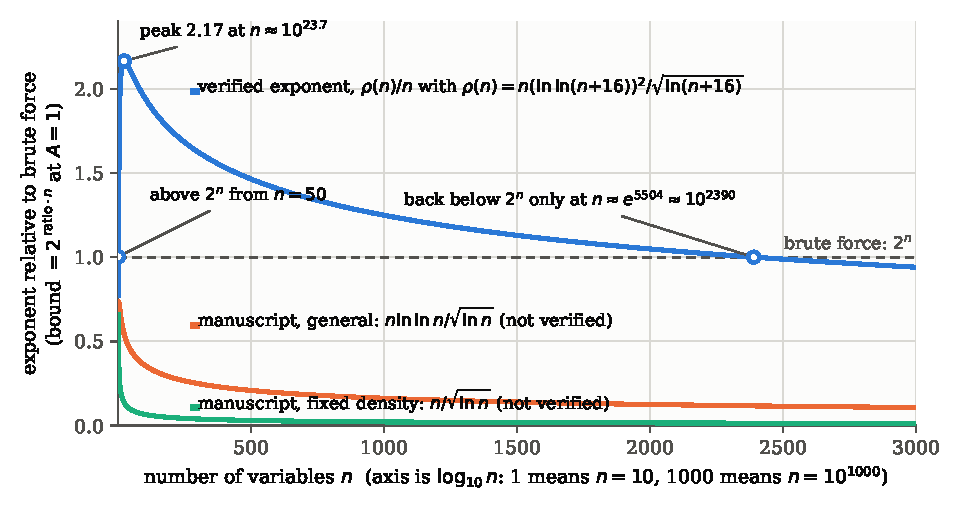
\includegraphics[width=\linewidth]{rho_over_n.pdf}\\[4pt]
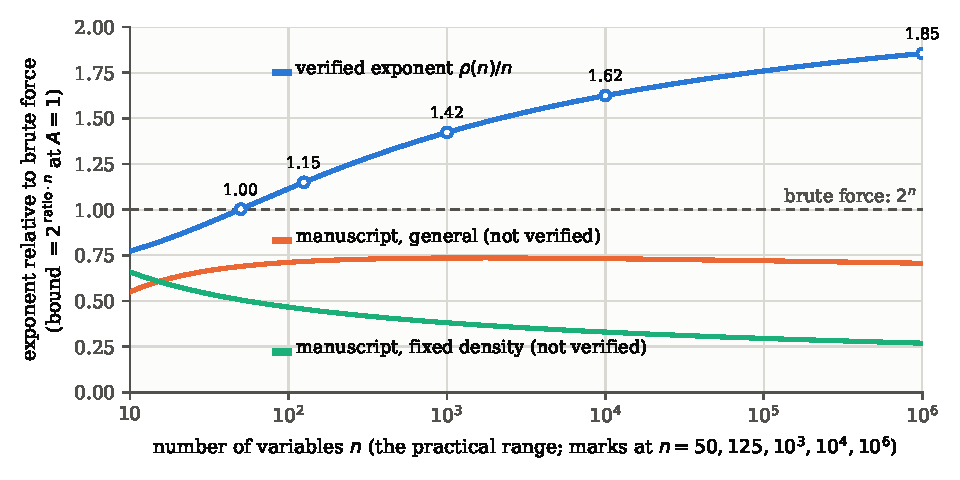
\includegraphics[width=\linewidth]{rho_over_n_practical.pdf}
\caption{The verified exponent against trying every assignment. Each
curve is an exponent divided by $n$; the dashed line at $1$ is $2^n$,
the cost of trying every assignment, and a curve above the line is a
guarantee worse than that. Top: the whole range, the horizontal axis
being the number of digits of $n$, from $n = 10$ to $n = 10^{3000}$.
The solid curve is the verified exponent $\rhon/n$; the two curves
beneath it are the manuscript's two sharper exponents,
$n\ln\ln n/\sqrt{\ln n}$ (the manuscript's Theorem~1.1, general case) and $n/\sqrt{\ln n}$ (its fixed-clause-density case), which are not in the Lean library
(Section~\ref{sec:beyond}). Bottom: the same three curves over the
practical range $n = 10$ to $10^6$, with $\rhon/n$ marked at $n = 50,
125, 10^3, 10^4, 10^6$. All curves take the constant $A$ to be $1$; the
verified $A$ is unknown and at least 257 in the proof on record.
Regenerate: \texttt{python3 -I paper3/scripts/rho\_over\_n.py}.}
\label{fig:central}
\end{figure}

\begin{figure}[htbp]
\centering
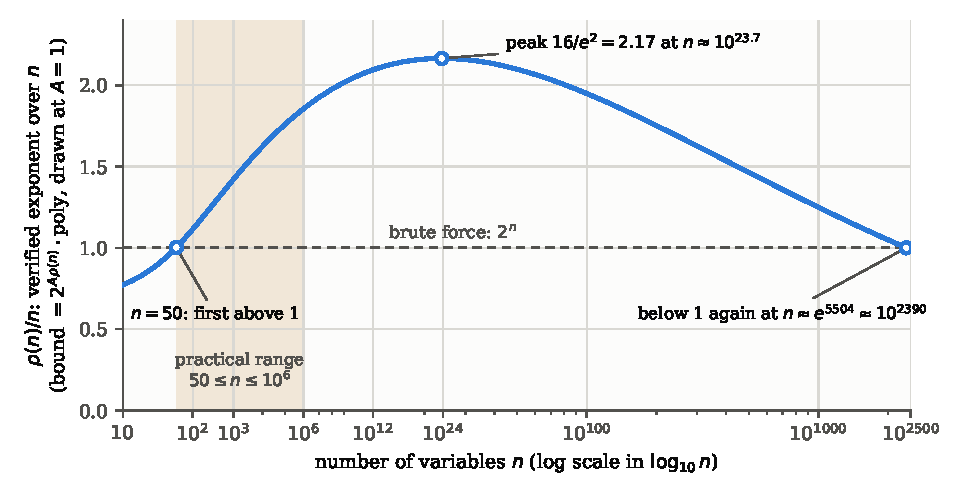
\includegraphics[width=\linewidth]{runtime_scale.pdf}
\caption{The ratio $\rhon/n$ alone, over an enormous range: the
horizontal axis is the number of digits of $n$, from $n = 10$ to
$n = 10^{2500}$. The level $1$ is the cost of trying every assignment.
Marked: the first whole number above the level ($n = 50$); the peak
($16/e^2 = 2.17$, at $n \approx 10^{23.7}$); the return below the level
($n \approx e^{5504} \approx 10^{2390}$); and, shaded, the practical
range $50 \le n \le 10^6$. Regenerate:
\texttt{python3 -I paper3/scripts/runtime\_scale.py}.}
\label{fig:runtime-scale}
\end{figure}

\subsection{The title's claim, made precise}
\label{sec:statement-title}

The title says the verified algorithm is slower than trying all $2^n$
assignments at every practical size. Read against the theorem, that
means the following four things, and nothing more.

\begin{enumerate}
\item \textbf{What is verified is a guarantee, not a running time.} The
  theorem says the machine halts within $C(L+1)^d\,2^{A\rhon}$ steps.
  It does not say how many steps the machine actually takes on any
  input. No implementation of the machine exists to be timed. A bound
  above $2^n$ does not say the machine is slow; it says the proof
  promises nothing better than $2^n$ there.
\item \textbf{The constants are never computed.} The theorem asserts
  that $C, A, S, d, e$ exist. The proof builds them from other
  existence lemmas and states no value, beyond the $A \ge 257$ read
  above. The machine's number of states is likewise never computed.
\item \textbf{With $A = 1$, the verified exponent is above $n$ for every
  $n$ from 50 up to about $10^{2390}$.} That is
  Table~\ref{tab:runtime-scale}. Over that range the exponential part
  of the bound is at least $2^n$, and at its worst it is $2^{2.17\,n}$.
  With the true $A$, whatever it is, the exponential part is $2^{A\rhon}$,
  which is at least $2^{\rhon}$ as soon as $A \ge 1$; and the proof's
  own construction has $A \ge 257$. So nothing on record puts the bound
  below $2^n$ at any practical size.
\item \textbf{Hence, at every practical size, the verified guarantee is
  weaker than the guarantee of trying all assignments.} Trying all
  $2^n$ assignments and checking each against the $m$ clauses counts
  the satisfying ones in $2^n$ times a small polynomial in $n + m$
  steps, with constants one can write down. The verified guarantee is
  $C(L+1)^d\,2^{A\rhon}$ with $\rhon > n$ on $50 \le n < e^{5504}$ and
  $C, A, d$ unknown. For every $C \ge 1$, $A \ge 1$ and $d \ge 1$ the
  verified bound is above $2^n$ on every $n$ in that range. The only
  values on record are the proof's own, which has $1 \le C$ and
  $1 \le A$ in the statement of its main run
  (\clonefile{SqrtLogSpace/NativeLargeEntry.lean}, line 12) and
  $A \ge 257$ in its construction. A proof with $A < 1$ would be a
  different proof; none is on record.
\end{enumerate}

None of this is a defect of the formalisation or of the proof. It is
what a theorem of this shape means when the constants in it are not
tracked. The manuscript itself calls $\rhon$ ``the weaker exponent''
(p.~2, line~63), and its sharper exponents are not in the Lean library
(Section~\ref{sec:beyond}). One detail of bookkeeping: inside the
solution the exponent is written with base-2 logarithms, and a lemma shows the two forms differ only by a fixed multiplier, which can be folded into the constant $A$ (Appendix~\ref{app:tech-theorem}); nothing above depends on it.

\subsection{What the statement does establish}
\label{sec:statement-establishes}

For each fixed width $k \ge 2$, there is a deterministic machine that,
given any $k$-CNF on $n$ variables with $m$ clauses in the fixed
encoding, halts with the exact number of satisfying assignments written
in binary on a named tape, within $C(L+1)^d\,2^{A\rhon}$ steps. Here
$L$ grows no faster than a polynomial in $n + m$, and $\rhon$ grows more
slowly than $n$. A formula of width $k$ on $n$ variables cannot have
more than about $n^k$ distinct clauses ($2{,}604{,}376$ at $n = 125$,
$k = 3$; Appendix~\ref{app:tech-theorem}), so the whole bound is
subexponential in $n$ alone. In the standard vocabulary, where $o(n)$ means a quantity that grows more slowly than $n$ and $\mathrm{poly}$ a polynomial: a deterministic $2^{o(n)} \cdot \mathrm{poly}(n+m)$ algorithm for counting the solutions
of $k$-SAT, and therefore for deciding it. That refutes the Exponential
Time Hypothesis \citep{ImpagliazzoPaturi2001}, the conjecture that
3-SAT needs time exponential in $n$, as stated. The verified theorem is
the manuscript's own verified form, the weaker exponent of its
Proposition~6.4 (p.~43, lines 2474--2476), without the $n \ge 20$
condition. We found no field, definition or quantifier through which
the statement could be accepted by the kernel and yet mean something
weaker than this; the audit behind that sentence is
\repofile{reports/scratch/eth_audit/statement_audit.md}. Our own
restatement of the theorem as a named Lean sentence, over a verbatim
copy of the machine model, is \leanref{subexpcount}; it is never proved
and never assumed there (Section~\ref{sec:lean}).

\subsection{What this does not claim}
\label{sec:statement-not}

\begin{itemize}
\item \textbf{No running time of any machine.} Nothing here measures or
  estimates how long the verified machine, or any program, takes on any
  input. The title compares two \emph{guarantees}.
  Section~\ref{sec:practitioner} is the only place in the paper where
  anything is timed, and it times ordinary solvers, not this machine.
\item \textbf{No statement about the proof.} That the statement means
  what we say it means is a reading of 220 lines. Whether the proof is
  sound is Section~\ref{sec:proof} and Section~\ref{sec:replay}, which
  found no flaw. The one proof-side fact quoted here, $A = 256 + A_t$,
  is a line of the solution read for the value it assigns, not a claim
  about the argument.
\item \textbf{No value of the constants.} $A \ge 257$ is what the proof
  writes down, not what the machine needs; a different proof of the
  same statement could have any $A > 0$. The statement itself fixes
  nothing.
\item \textbf{Nothing about the manuscript's sharper exponents}, which
  are not in the Lean library and are Section~\ref{sec:beyond}'s
  subject.
\item \textbf{No claim about sizes beyond $e^{5504}$.} Past
  $n \approx 10^{2390}$ the verified exponent is below $n$ again at
  $A = 1$; we say nothing about that range except that it is not a
  practical one.
\end{itemize}
\par\endgroup

% What the manuscript claims beyond the verified statement -- drafted by loop0015 item 03.
\section{What the manuscript claims beyond the verified statement}
\label{sec:beyond}

\placeholder{Item 03 drafts this section: Theorem 1.1's two sharper exponents, Corollary 1.4's quantitative circuit bound, Appendix C's consequences, Appendix D, each tagged verified or paper-only with page and line of the extract. Ends with what this does not claim''.}

% The proof, inspected -- drafted by loop0015 item 04 (2026-11-05). Every
% number of this section is printed, and every line citation re-checked
% against the read-only clone at commit 4eaee875, by
%   python3 -I paper3/scripts/proof_inspection.py
% which re-runs the two audit scripts of reports/scratch/eth_audit/
% (closure.py, defdiff.py) as subprocesses, performs the remaining checks
% itself, writes latex/tables/proof_inspection.tex, and exits non-zero if
% anything has moved. Unqualified Lean paths below are relative to
% lean/OAI/Algorithms/SubexponentialSAT/ in the clone; the challenge file is
% lean/ComparatorChallenges/SubexponentialSAT.lean. Nothing in the clone was
% built, imported or run for this section; the build is Section 5's.
\section{The proof, inspected}
\label{sec:proof}
\begingroup\sloppy

Section~\ref{sec:statement} read the theorem; this section reads the
proof, as far as reading can go. The question is not whether the
mathematics is right---the kernel decides that, and Section~\ref{sec:replay}
reports what the kernel said when we ran it---but whether anything in the
source could make the kernel's acceptance mean less than it appears to
mean: an axiom, a \texttt{sorry}, a trusted evaluation, an unsound
instance, a patched Mathlib, a statement that differs from the challenge's,
or a cost model of the proof's own that leaks into the theorem. We found
none of these. What we did find is that the repository offers no recorded
evidence that the closure type-checks at all---no \texttt{\#print axioms}
output, no continuous integration, no second kernel for this family---which
is why Section~\ref{sec:replay} exists. The last subsection joins the two.

\subsection{Method}
\label{sec:proof-method}

The clone of \texttt{openai/math} at commit \texttt{4eaee875} is treated as
untrusted data: every file was read with \texttt{cat}, \texttt{sed},
\texttt{grep} and \texttt{python3 -I}, and nothing in it was built,
imported or executed for this section. Two scripts from the audit of
2026-11-05 do the mechanical part: \texttt{closure.py} follows
\texttt{import} lines from the solution module, strips comments (nested
block comments included) and counts keyword occurrences in what remains;
\texttt{defdiff.py} normalises whitespace and compares each declaration of
the challenge file with the library's declaration of the same name. Both
were re-run for this section, and every number below is from that fresh
run; \repofile{paper3/scripts/proof_inspection.py} re-runs them, performs
the remaining checks, and regenerates Table~\ref{tab:proof-inspection}.
The inspection is of the spine of the proof---the final file, the
compiler, the entry lemmas, the constants---and of the whole closure by
keyword. The arithmetic beneath the spine was not read
(Section~\ref{sec:proof-not}).

\subsection{The closure}
\label{sec:proof-closure}

The comparator's JSON names one solution module,
\path{OAI.Algorithms.SubexponentialSAT.Main}, a sixteen-line aggregator
that imports \texttt{SqrtLog.ExecutionNativeFinal} and
\texttt{SqrtLogSpace.Final} and declares nothing
(\clonefile{Main.lean}). Its import closure inside the repository is
\textbf{3,091 modules}, every one with the prefix
\path{OAI.Algorithms.SubexponentialSAT}, totalling \textbf{550,551} raw
lines; the largest file is 2,873 lines
(\clonefile{SqrtLogSpace/DisjointReuse/SparsePriorityProgram.lean}). The
closure stops at \textbf{50} Mathlib modules and one module of Lean's own
library, \path{Lean.Elab.Tactic.Omega}, imported by
\clonefile{SqrtLogSpace/FiniteFallback.lean} (line~14) and
\clonefile{SqrtLogSpace/DisjointReuse/SparseCharging.lean} (line~5); it
is a tactic module, and the closure defines no tactic, macro or syntax of
its own (Section~\ref{sec:proof-keywords}). Nothing is imported from any
other family of the collection or from any of the repository's other
dependencies.

The family's directory holds \textbf{3,977} \texttt{.lean} files, so
\textbf{886} are outside the closure. They are not reachable from the
collection's root module either: \clonefile{lean/OAI.lean} imports the
family only at its line~49, \texttt{import} \path{OAI.Algorithms.SubexponentialSAT.Main}, and the lakefile's default target
is that root (\clonefile{lean/lakefile.lean}, line~89,
\texttt{@[default\_target] lean\_lib OAI}). They are therefore never built
by the default target and bear on nothing: dead files, not a hole. For
completeness, a raw search of the 886 for \texttt{sorry}, \texttt{axiom},
\texttt{native\_decide} and \texttt{admit} finds nothing, with or without
comments.

\subsection{The keyword sweep}
\label{sec:proof-keywords}

Table~\ref{tab:proof-inspection} gives the counts over the 3,091 files
with comments stripped. The ones that matter are the zeros. There is no
\texttt{axiom}, no \texttt{sorry}, no \texttt{admit}; no
\texttt{native\_decide} and no \texttt{ofReduceBool}, so nothing is
proved by trusting the compiled evaluator; no \texttt{implemented\_by},
\texttt{extern}, \texttt{unsafe} or \texttt{partial}, so no definition
has a hidden implementation and every recursion is one the kernel checks
(nine \texttt{termination\_by} and five \texttt{decreasing\_by} clauses);
no \texttt{elab}, \texttt{macro}, \texttt{syntax} or \texttt{simproc}, so
there is no metaprogramming that could rewrite goals outside the kernel's
view. The only \texttt{set\_option}s are two
\texttt{set\_option quotPrecheck false}
(\clonefile{SqrtLog/LeafProgramPreparedRecoveryQuery.lean}, line~15, and
\clonefile{SqrtLog/LeafProgramPreparedRecoveryWitness.lean}, line~14),
which switch off a pre-check on local notation and have no bearing on
soundness; there is no \texttt{maxHeartbeats}, \texttt{maxRecDepth} or
\texttt{autoImplicit} option anywhere in the closure, and the lakefile
sets \texttt{autoImplicit} to \texttt{false} for the whole package
(\clonefile{lean/lakefile.lean}, line~9).

Nine declarations are \texttt{opaque}, and every one carries a body:
\begin{itemize}
\item three recovery functions: \texttt{queryRecovery} at line~59 of
  \clonefile{SqrtLog/LeafProgramPreparedRecoveryQuery.lean}, with its
  \texttt{:= by} at line~86; \texttt{rawRecovery} and
  \texttt{fixedRecovery} at lines 178 and 198 of
  \clonefile{SqrtLog/LeafProgramPreparedRecoveryWitness.lean};
\item six \texttt{private opaque} constants of a subtype
  \texttt{\{ports // ports = \ldots\}}, each with an explicit value:
  line~22 of \clonefile{SqrtLog/LeafProgramQueryCleanup.lean} and five
  others.
\end{itemize}
An \texttt{opaque} with a body is a definition whose unfolding
is hidden from elaboration; the kernel still checks the body against the
type, so nothing is assumed. The 1,048 \texttt{noncomputable}
declarations, the eight \texttt{open Classical}, and the four explicit
uses each of \texttt{Classical.choice} and \texttt{propext} are the
classical reasoning the comparator permits. The 148 \texttt{instance}s
and 40 \texttt{local instance}s are \texttt{Fintype},
\texttt{Decidable} and algebraic instances; an instance cannot be
``inconsistent'' without an axiom, and there is none. The 14,034 lines
with \texttt{decide} are kernel-evaluated decision procedures, not the
native evaluator.

\begin{table}[t]
\centering\small
\caption{The inspection in numbers. Comments stripped where a keyword is
counted. Regenerate: \texttt{python3 -I paper3/scripts/proof\_inspection.py}.}
\label{tab:proof-inspection}
% Generated by python3 -I paper3/scripts/proof_inspection.py -- do not edit.
\begin{tabular}{@{}p{0.50\linewidth}p{0.17\linewidth}p{0.25\linewidth}@{}}
\toprule
quantity & value & script \\
\midrule
modules in the closure of \texttt{Main.lean} & 3,091 & \texttt{closure.py} \\
raw lines in those modules & 550,551 & \texttt{closure.py} \\
external imports: Mathlib modules / core modules & 50 / 1 & \texttt{closure.py} \\
\texttt{.lean} files under the family / outside the closure & 3,977 / 886 & this script \\
\texttt{axiom}, \texttt{sorry}, \texttt{admit}, \texttt{native\_decide}, \texttt{ofReduceBool} & 0, 0, 0, 0, 0 & \texttt{closure.py} \\
\texttt{implemented\_by}, \texttt{extern}, \texttt{unsafe}, \texttt{partial} & 0, 0, 0, 0 & \texttt{closure.py} \\
\texttt{elab}, \texttt{macro}, \texttt{syntax}, \texttt{simproc} & 0, 0, 0, 0 & \texttt{closure.py} \\
\texttt{set\_option} (both \texttt{quotPrecheck false}) & 2 & \texttt{closure.py} \\
\texttt{opaque} (all with bodies) & 9 (9) & \texttt{closure.py}, this script \\
\texttt{noncomputable} & 1,048 & \texttt{closure.py} \\
explicit \texttt{Classical.choice} / \texttt{propext} / \texttt{open Classical} & 4 / 4 / 8 & \texttt{closure.py} \\
\texttt{instance} / \texttt{local instance} & 148 / 40 & \texttt{closure.py} \\
\texttt{termination\_by} / \texttt{decreasing\_by} & 9 / 5 & \texttt{closure.py} \\
statement definitions compared / identical / identical up to \texttt{noncomputable} & 35 / 33 / 2 & \texttt{defdiff.py}, this script \\
theorem statement, characters (normalised / raw), identical & 1,124 / 1,353 & this script \\
\texttt{\#print axioms} commands: closure files / lines; family files / lines & 8 / 19; 17 / 35 & this script \\
recorded \texttt{depends on axioms} outputs in the clone & 0 & this script \\
challenge JSONs: total / \texttt{enable\_nanoda} false / true / absent & 418 / 413 / 2 / 3 & this script \\
CI workflow files (\texttt{lock-prs.yml} only) & 1 & this script \\
manifest packages / patch files / patches for Mathlib & 42 / 23 / 0 & this script \\
\bottomrule
\end{tabular}

\end{table}

\subsection{The statement is the challenge's}
\label{sec:proof-match}

The solution file does not import the challenge file:
\clonefile{SqrtLogSpace/Final.lean} begins (lines 1--3) with
\texttt{NativeLargeEntry}, \texttt{SqrtLogSpace.Statement} and
\texttt{SqrtLog.StatementCanonical}. The library re-declares every
definition the statement uses under the same fully qualified names,
spread over seven files: the SAT vocabulary in \clonefile{SAT.lean}, the
bit arithmetic in \clonefile{BinaryArithmetic.lean}, the nine encoding
functions in \clonefile{Encoding.lean}, the machine in
\clonefile{Computation.lean}, \texttt{runtimeScale} and
\texttt{runtimeBound} in \clonefile{SqrtLog/StatementScale.lean}, the
space instrumentation in \clonefile{SqrtLogSpace/VisitedTape.lean} and
\texttt{countWord} in \clonefile{SqrtLogSpace/EncodingBounds.lean}
(line~17, the challenge's line~147). The definition diff compares
\textbf{35} declarations: \textbf{33} are identical character for
character after whitespace normalisation, and the remaining two,
\texttt{runtimeScale} and \texttt{runtimeBound}, differ only in that the
challenge writes \texttt{noncomputable def} where the library opens a
\texttt{noncomputable section} (\clonefile{SqrtLog/StatementScale.lean},
line~15)---a difference the kernel does not see. The theorem statement
itself, from \texttt{theorem exact\_count\_and\_sat} to \texttt{:= by},
is \textbf{identical} in the two files, 1,353 characters raw and 1,124
after normalisation, at line~194 of the challenge and line~74 of
\clonefile{SqrtLogSpace/Final.lean}; the challenge's proof is the single
word \texttt{sorry} at its line~218.

This textual match is a sanity check and not the guarantee. The
comparator \citep{LeanComparator} compares the two statements at the
level of exported constants, with every declaration the statement
mentions matched, so a library definition that differed from the
challenge's under the same name would make the comparator fail rather
than pass silently. What the text confirms is that there is no such
difference to find, and that the shape Section~\ref{sec:statement} read
is the shape the library proves.

\subsection{The spine of the proof}
\label{sec:proof-spine}

\paragraph{The machine.} The theorem's machine is
\texttt{GuardedCompiler.primitive program} with the count tape
\texttt{256} and the answer tape \texttt{1216} (both \texttt{: Fin 1220};
\clonefile{SqrtLogSpace/Final.lean}, line~100), where \texttt{program}
is \texttt{Native.countingProgram cutoff k} \texttt{(NativeLeafProgram.command k)}
(line~40), a \texttt{BitProgram.Program 80 1220 labels} (line~11): a
first-order program over 80 one-bit registers, 1,220 Boolean stacks and
a finite label set, with twelve instruction kinds
(\clonefile{BitProgram.lean}, lines 10--26). \texttt{primitive}
(\clonefile{SqrtLogSpace/GuardedCompiler.lean}, line~131) is a
\texttt{noncomputable abbrev}: it takes the transition table
\texttt{transition p} (lines 30--47, one case per instruction) and the
stack selector \texttt{selected p} (lines 14--17), feeds them to the
stack compiler's controller, and renames the finite state type to
\texttt{Fin stateCount} through \texttt{Fintype.equivFin} (line~132).
The machine is thus a concrete table defined by pattern matching on the
program, composed with a classical renaming of states; the theorem is
existential, so the noncomputability costs it nothing, and it is the
reason no running time can be read off the statement
(Section~\ref{sec:statement}).

\paragraph{The time bound, and the constants.} For \texttt{cutoff < n},
\path{NativeLargeEntry.run} (\clonefile{SqrtLogSpace/NativeLargeEntry.lean},
lines 11--33) supplies a trace of length at most
\texttt{runtimeBound C A d L n} (line~27) with $1 \le C \wedge 1 \le A$
(line~12). Its exponent constant is \texttt{256 + At} (line~51), where
\texttt{At} comes from the leaf program's uniform contract
(\path{NativeLeafContract.uniform_contract}, line~39; the contract
gives $1 \le \mathtt{At}$, \clonefile{SqrtLogSpace/NativeLeafContract.lean},
line~793), and its cutoff is \texttt{max 20 (max Nleaf Ns)} (line~50),
with \texttt{Ns} obtained non-constructively from an eventual inequality
(\path{Filter.eventually_atTop}, line~48). The $2^{A\cdot\mathtt{runtimeScale}\,n}$
factor is assembled by \path{runtime_of_tree_and_leaf} (line~46)
from the DFS visit bound of \path{Native.outer_from_setup}
(\clonefile{SqrtLogSpace/NativeOuter.lean}, lines 53--56: visits at most
a square polynomial in $n$ times $2^{n/\mathtt{sparsifySchedule}\,n}$)
and the leaf time. For $n \le \mathtt{cutoff}$,
\path{Native.entry_small_primitive}
(\clonefile{SqrtLogSpace/NativeEntry.lean}, lines 81--100) gives
$\mathtt{time} \le 28700\,(L+1)^2$ (line~92) through the finite scanner
of \clonefile{SqrtLogSpace/FiniteFallback.lean}. The two branches are
folded by \texttt{runtime\_with\_fallback} and
\texttt{space\_with\_fallback}
(\clonefile{SqrtLogSpace/NativeOuterBudgets.lean}, lines 297 and 317)
into one triple, and the witnesses the final theorem exhibits are
\texttt{C + 28700, A + 1, S + 5022741, d + 2, e + 2}
(\clonefile{SqrtLogSpace/Final.lean}, line~41). So the proof as written
has an exponent constant of at least $258$ in front of $\rhon$, a
polynomial degree \texttt{d} that depends on $k$ (line~51: $\mathtt{db} + (4(k-2)+2) + \mathtt{df} + 2$) and a leading constant of at least
$28{,}701$; none of these is in the statement, which asserts only that
they are positive, and none of \texttt{At}, \texttt{db}, \texttt{df} is
computed anywhere. This confirms, from the proof side, what
Section~\ref{sec:statement} said from the statement side: the constants
are unknown, and the \emph{smallest} they could be is already far from
$1$.

\paragraph{Where a hidden cost model would live, and why it cannot.}
A proof of a running-time bound for a machine it compiles from a
higher-level program could, in principle, prove the bound against a cost
function of its own and leave the kernel to check only that function's
arithmetic. That is not what happens here. The compile lemmas conclude in
the comparator's own vocabulary: \path{GuardedCompiler.primitive_execution}
(\clonefile{SqrtLogSpace/GuardedCompiler.lean}, lines 158--162) turns a
source run of \texttt{n} steps into \texttt{RunsIn (primitive p).step
(7 * n)}, with the overhead \texttt{7} proved as a theorem
(\texttt{compiler\_overhead}, lines 152--153), and
\path{CompileSpace.compile_word_answer_space}
(\clonefile{SqrtLogSpace/CompileSpace.lean}, lines 125--143) produces a
\texttt{Computation.Trace (locatedStep (primitive p)) time \ldots} with
$\mathtt{time} \le 7\cdot\mathtt{sourceSteps}$ and
$\mathtt{visitedSpace}\ \mathtt{intermediate} \le s\,(\mathtt{bound} + \mathtt{input.length} + 15)$ on
every prefix (lines 134, 135 and 143); \path{primitive_located_step}
(\clonefile{SqrtLogSpace/GuardedCompiler.lean}, line~600) is the per-step
form. \texttt{Trace}, \texttt{locatedStep} and \texttt{visitedSpace} are
the challenge's definitions (its lines 87--90 and 149--189), and
\texttt{time} in the final theorem is literally the length of a
\texttt{Computation.Trace} of \texttt{PrimitiveMachine.step} (its
line~201). No cost function of the compiler's appears in the statement;
a wrong cost model would make these lemmas unprovable, not the theorem
false. This is the structural point on which the rest of the paper
leans: whatever the proof's internal accounting, the number the theorem
bounds is the number of steps of the comparator's machine.

\paragraph{Correctness of the count.} \path{Native.outer_from_setup}
(\clonefile{SqrtLogSpace/NativeOuter.lean}, lines 50--51) yields
\texttt{final.stacks ABI.countStack = countWord (SAT.count F)} and
\texttt{final.stacks ABI.answerStack = [decide (0 < SAT.count F)]} from
the canonical DFS execution, and
\path{Native.counting_primitive_from_entry} (line~73) transports
both to the primitive machine's tapes; \texttt{countWord\_toNat} and
\texttt{countWord\_count\_length} supply the decoding and length clauses
of the statement. These are theorems about the concrete step function.
The arithmetic that makes them true---sparsification, the ring and
moment computations, the DFS---is the content of the other three
thousand files, and the only claim made about it here is the one the
kernel makes: it elaborates (Section~\ref{sec:replay}).

\subsection{Toolchain, Mathlib, and the build hooks}
\label{sec:proof-build}

The toolchain is fixed (\clonefile{lean/lean-toolchain}:
\texttt{leanprover/lean4:v4.34.1}; \clonefile{lean/lakefile.lean}
line~8: \texttt{fixedToolchain := true}). The manifest lists 42
packages; Mathlib is pinned to upstream revision
\texttt{d13f23b723b8a846827a245b89c10fc7d3f11612} at
\path{leanprover-community/mathlib4}, and the audit of 2026-11-05
confirmed that revision on GitHub as the upstream commit that bumps the
toolchain to \texttt{v4.34.1}. The repository carries 23 compatibility
patches under \clonefile{lean/patches/}, \textbf{none for Mathlib};
every one is for a third-party package (\texttt{AINTLIB},
\texttt{PrimeNumberTheoremAnd}, \texttt{carleson}, \texttt{iut}, \ldots) that
this closure does not import. The lakefile has two hooks that run
arbitrary IO when Lake configures or updates the package: a
\texttt{run\_cmd} block (lines 290--304) that evaluates dependency
declarations with \texttt{unsafe env.evalConstCheck} and calls
\path{preparePatchedDependencies}, which clones and patches eleven
dependencies, and a \texttt{post\_update} hook (line~306 onward) that
verifies or applies the patches for the rest. They touch only
\texttt{.lake/packages}, and only non-Mathlib packages; they are one
reason the inspection did not build, and the reason the replay of
Section~\ref{sec:replay} runs inside a sandbox with the network on.

\subsection{What the repository does not record}
\label{sec:proof-missing}

Three things one would expect beside a verified refutation of a
forty-year-old hypothesis are absent, and their absence is a fact about
evidence rather than about the proof.

\begin{itemize}
\item \textbf{No axiom audit.} \clonefile{SqrtLogSpace/Final.lean} ends
  with five \texttt{\#print axioms} commands (lines 197--201), and seven
  other files of the closure carry fourteen more (nineteen commands in
  eight files; the family's directory holds seventeen such files, but
  nine of them are among the 886 never built). Their output exists only
  while the build runs and is recorded nowhere: a search of the whole
  clone for the string \texttt{depends on axioms} finds nothing.
\item \textbf{No continuous integration.} \clonefile{.github/workflows/}
  holds one file, \texttt{lock-prs.yml}, which locks pull-request
  conversations. Nothing builds or checks the Lean.
\item \textbf{No second kernel for this family.} The comparator's JSON
  (\clonefile{lean/ComparatorChallenges/SubexponentialSAT.json}) names the
  one theorem, an empty \texttt{definition\_names}, the three permitted
  axioms \texttt{propext}, \texttt{Quot.sound}, \texttt{Classical.choice},
  and \texttt{enable\_nanoda: false}; the registry
  \clonefile{lean/formalization.yaml} (lines 1683--1685) points at the
  same declaration and file. Of the collection's 418 challenge JSONs,
  413 set \texttt{enable\_nanoda} to \texttt{false}, two to
  \texttt{true}, and three omit the key. With it off, the collection's own
  check of this family rests on one kernel implementation. The
  comparator's README, as fetched by the audit, describes the check as:
  build challenge and solution in a sandbox, export both with
  \texttt{lean4export}, match each named theorem's statement with every
  declaration it uses, confine the proof to the permitted axioms, and
  have the Lean kernel accept it; with nanoda on, the exported
  environment is replayed through an independent kernel in Rust as well
  \citep{Nanoda}. Section~\ref{sec:related} records the versions.
\end{itemize}

Two smaller consistency facts, for the record. The manuscript's source is
dated ``17 October 2026, revised 25 October 2026''
(\clonefile{preprints/The-Exponential-Time-Hypothesis-is-False-October-25-2026/build/main_full_version.tex}, line~25); the
collection's history file mentions the family once, in the sentence that
names the working group at whose request the materials were released
(\clonefile{history.md}, line~18), and its only ``Formalization Fix''
entry (line~7) concerns another family. And the scope note
\clonefile{lean/docs/378.md} states the verified exponent as
$n(\log\log n)^2/\sqrt{\log n}$ (line~9), which is what the library
proves and what Section~\ref{sec:beyond} compares with the manuscript's.

\subsection{The trust boundary, joined with the replay}
\label{sec:proof-trust}

The audit's verdict listed what the proof's trust rested on before
anything was run: (i) OpenAI's unpublished build, since nothing showed
the closure type-checks; (ii) the absence of any recorded axiom output;
(iii) the Lean kernel of \texttt{v4.34.1} and Mathlib \texttt{d13f23b7}
as upstream; (iv) the comparator run, not reproduced; (v) no second
kernel for this family. Table~\ref{tab:proof-trust} says which of the
five Section~\ref{sec:replay} moved.

\begin{table}[t]
\centering\small
\caption{The trust boundary before and after the replay of
Section~\ref{sec:replay}.}
\label{tab:proof-trust}
\begin{tabular}{@{}p{0.30\linewidth}p{0.64\linewidth}@{}}
\toprule
item & status after the replay \\
\midrule
(i) the build & \textbf{moved}: the 3,091-module closure built from source in our sandbox at the pinned toolchain, exit~0, no \texttt{error}, no \texttt{sorry}. \\
(ii) the axiom output & \textbf{moved}: \texttt{\#print axioms} of the comparator's theorem printed \texttt{[propext, Classical.choice, Quot.sound]}, and the nineteen in-build axiom lines say the same; the output is on record. \\
(iii) kernel and Mathlib & \textbf{moved in part}: Mathlib was fetched from upstream at the pinned revision and not patched, so ``as upstream'' is now observed rather than assumed; the Lean kernel of \texttt{v4.34.1} is still trusted as upstream, now beside a second kernel (v). \\
(iv) the comparator run & \textbf{not moved}: the statement-level match through \texttt{lean4export} was not performed; the match this paper relies on is the textual one of Section~\ref{sec:proof-match}. \\
(v) a second kernel & \textbf{moved}: \texttt{nanoda\_lib} checked the exported dependencies of the theorem, 95,176 declarations, with no errors and the three axioms; what this adds and what it does not is stated in Section~\ref{sec:replay}. \\
\bottomrule
\end{tabular}
\end{table}

After the replay, then, the proof's trust rests on: the Lean kernel of
\texttt{v4.34.1} \emph{and} nanoda agreeing on the exported dependencies
of the theorem; \texttt{lean4export} exporting what the environment
holds; upstream Mathlib at the pinned revision; and the textual, not
export-level, match between the solution's statement and the
challenge's. Everything the inspection could find by reading, the build
and the two kernels confirmed; nothing the inspection could not settle
by reading has been settled by anything else.

\subsection{What this does not claim}
\label{sec:proof-not}

\begin{itemize}
\item \textbf{The arithmetic was not read.} The inspection followed the
  spine from \clonefile{SqrtLogSpace/Final.lean} down to the compile
  lemmas and swept the whole closure by keyword; the sparsification, ring
  and DFS content of the other three thousand files was not read. The
  argument above is that its correctness is kernel-enforced, not that we
  verified it.
\item \textbf{Grep is necessary, not sufficient.} Zero \texttt{sorry}
  and zero \texttt{axiom} by text search cannot show that a file
  elaborates; only the build does (Section~\ref{sec:replay}). Conversely
  a keyword count is over source text at one commit, and a declaration
  can be unsound only through the mechanisms searched for; we searched
  for the ones we know.
\item \textbf{The textual statement match is not the comparator's.} The
  comparator matches exported constants; we matched source text after
  whitespace normalisation and found it identical. A difference the
  normalisation hides would have to be invisible to the kernel as well,
  but that is an argument, not a run.
\item \textbf{Nothing about the constants' values.} The bounds
  $A \ge 258$ and $C \ge 28{,}701$ are what the proof's witnesses are
  built from; they are lower bounds on what this proof exhibits, not
  statements about any machine's running time, and a different proof of
  the same statement could exhibit different ones.
\item \textbf{Nothing about the Lean kernel, Mathlib or the toolchain.}
  All three are trusted as upstream at the pinned versions; the second
  kernel of Section~\ref{sec:replay} is evidence about the first, not a
  proof of either.
\item \textbf{Nothing about what the theorem says.} That is
  Section~\ref{sec:statement}; a sound proof of a weak bound is a sound
  proof of a weak bound.
\end{itemize}
\par\endgroup

% Independent replay -- drafted by loop0015 item 01.
\section{Independent replay}
\label{sec:replay}

\placeholder{Item 01 drafts this section: the sandboxed build of the SubexponentialSAT closure from a fresh copy of the clone, the \texttt{\#print axioms} output, the Lean and Mathlib versions, the time, the hashes of the logs, and whether nanoda ran. Ends with what this does not claim''.}

% What follows -- drafted by loop0015 item 05.
\section{What follows}
\label{sec:consequences}

\placeholder{Item 05 drafts this section: which hypotheses the verified statement refutes (ETH, SETH, Gap-ETH, \#ETH, NSETH, the randomised forms) and how; in general terms, that a lower bound derived from ETH or SETH loses its premise while a statement ``no $(c-\varepsilon)^k$ algorithm'' is not itself refuted (the manuscript's \S1.1.3); no example from any width parameter. Ends with what this does not claim''.}

% For the practitioner -- drafted by loop0015 item 06.
\section{For the practitioner}
\label{sec:practitioner}

\placeholder{Item 06 drafts this section: a SAT solver and a model counter on random 3-CNF at $n = 20\ldots 60$ against $2^{\rhon}$ and $2^n$ (figure labelled \texttt{fig:practitioner}, from \repofile{paper3/scripts/practitioner.py}); the verified guarantee is never the binding one on any machine. Ends with what this does not claim''.}

% The statement in our Lean -- drafted by loop0015 item 07.
\section{The statement in our Lean}
\label{sec:lean}

\placeholder{Item 07 drafts this section: the restatement $\SubexpCount$ over the verbatim machine model under \repofile{lean/MOSPFormalization/ETH/}, the axiom audit, the byte-level re-diff against the comparator file; no theorem of ours about the hypothesis is proved, and none is claimed. Ends with what this does not claim''.}

% Related work and context -- drafted by loop0015 item 08.
\section{Related work and context}
\label{sec:related}

\placeholder{Item 08 drafts this section: the human audit of the August 2026 results (arXiv 2608.14673), the working group named in the collection's history, Impagliazzo--Paturi, Impagliazzo--Paturi--Zane, the comparator mechanism, nanoda; ``we found no prior statement'', never ``first''. Ends with what this does not claim''.}

% Conclusion -- drafted by loop0015 item 09 (2026-11-05), in plain English
% (owner's rule of 2026-11-05 05:30). The second subsection reviews every
% entry of paper3/ETH_AMBIGUOUS.MD written up to this section (S1-S8,
% 01a-08xd, and 09a-09d of this item) and lists the ones that affect the
% text as open, by entry number; the owner resolves an entry by editing the
% paper and striking it. Nothing here is a new number: every figure quoted
% is a later section's, with its section named.
\section{Conclusion}
\label{sec:conclusion}
\begingroup\sloppy

OpenAI's family 378 holds a theorem the Lean kernel accepts, and the
theorem refutes the Exponential Time Hypothesis as stated. We read it,
inspected its proof, rebuilt the proof from source and re-checked it
with a second checker, and found no flaw. That is the first thing this
paper says, and it is said without qualification. The second thing is
what the title says, and it is a reading of the statement, not of the
proof. The statement is a guarantee: a machine exists and halts within
a bound. The bound's constants exist and are never computed; where the proof
writes values down, its construction has at least 257 for the
exponent's constant, and the theorem it exhibits has at least 258
there and at least 28,701 in front (Sections~\ref{sec:statement} and
\ref{sec:proof}). The exponent is the manuscript's weaker one, and with
its constant set to one it exceeds the number of variables at every
size from 50 up to a number with 2,391 digits
(Section~\ref{sec:statement}). So at every practical size the verified
guarantee is weaker than the guarantee of trying every assignment. The
manuscript's sharper exponents, which would change that sentence, are
not in the Lean library (Section~\ref{sec:beyond}). What follows from
the verified statement is exactly what the manuscript says follows: the
hypotheses fall, the lower bounds derived from them lose their premise,
and the conclusions of those lower bounds are untouched
(Section~\ref{sec:consequences}). For anyone who runs a solver, nothing
changes (Section~\ref{sec:practitioner}). Two facts are true at
once, and neither diminishes the other. In the limit, the exponent is
smaller than the number of variables by any factor one names; that is
a theorem in our own Lean (Section~\ref{sec:lean}). On every size anyone
will write down, it is larger.

\subsection{What is claimed, and what is not}
\label{sec:conclusion-claims}

The introduction's two lists (Section~\ref{sec:intro-claims}) are the
paper's claims and non-claims, and each later section repeats its own
under ``what this does not claim''. In one sentence each. The verified
statement is a guarantee with uncomputed constants, above $2^n$ at every
practical size with the constants set to one, and it refutes ETH and its
relatives nonetheless. The proof shows no flaw by inspection, builds
from source, and passes two checkers. The sharper exponents are
paper-only. And no running time of any machine, no flaw in anything,
no value of any constant beyond the proof's own, and no refutation of
any derived lower bound's conclusion is asserted. Every number in the
paper has a script under \repofile{paper3/scripts/} that regenerates
it, every quotation has a page and line or a file and line, and the
replay's logs and hashes are under \repofile{paper3/replay/}.

\subsection{The questions this reading left open, by entry}
\label{sec:conclusion-open}

The paper was written under a rule that no question stops the work.
A choice between two sound ways of saying or doing a thing is made and
recorded in \repofile{paper3/ETH_AMBIGUOUS.MD} as one numbered entry.
The entry says what was ambiguous, what was chosen and what the author
may want to change. Then the writing goes on. Sixty-one entries were
written in all: forty-four before the first draft of this section,
four by that draft, eleven by the reading of the whole paper and the
write-up that followed it, and two by the final pass. We reviewed all
sixty-one and sort them here. Twenty-two need no decision. Seven were
resolved by the author in writing: S1, the author line; S3, where the
companion Lean lives, with 07a following it; S4, no width references;
S6, the model counters; S7, the phrase ``for every $50 \le n <
e^{5504}$''; S8, the replay's Lean version. Fifteen are procedural, or
are corrections the text already carries: S5, the per-item time cap of
the writing driver; 01a, the sandbox's core cap; 03b, the manuscript
has 67 pages; 04b, 04d and 04e, three counts corrected from an earlier
audit; 06b, a counter installed for Section~\ref{sec:practitioner};
08xb, which sections the plain-English rewrite covered; 10c, the long
sentences the first reading left, since split; 11c, two audit files
annotated rather than edited; 11d, the later entries listed in the
repository's README, and since here too; 11e, a paragraph for the
repository's instructions file, drafted and not applied; 11f, the
plan's record of what was done; 12a and 12b, the scope of the final
pass and this list's own re-count. The thirty-nine below affect the
text and are open. In each case the text stands as chosen, and the
entry says what would change.

\begin{description}\setlength{\itemsep}{1pt}
\item[The title and its figures.] S2: $2^n$ is typeset with a
  superscript and the ellipsis as three dots; the plain text is in the
  PDF's metadata. 02a: Section~\ref{sec:statement} carries both the
  two-panel Figure~\ref{fig:central} and Figure~\ref{fig:runtime-scale},
  three drawings of one function. 02b: the central figure's peak is
  placed analytically and its legend carries the $+16$. 10b: the
  title's ``is slower'' is reconciled with the paper's non-claim of any
  running time by Sections~\ref{sec:statement} and
  \ref{sec:practitioner}, and by nothing in the title itself.
\item[The statement (Section~\ref{sec:statement}).] 02c: a proof-side
  fact, the constant $256 + A_t$, is quoted in the statement section
  for its value. 02d: the Lean theorem is transcribed as a display, not
  shown verbatim, because the house build cannot typeset its symbols.
  08xd: Section~\ref{sec:statement} says the proof's constant is at
  least 257 and the exhibited theorem's at least 258, two readings of
  two lines, both kept.
\item[Beyond the statement (Section~\ref{sec:beyond}).] 03a: a third
  tag, ``supported'', between verified and paper-only. 03c: what the
  verified exponent would give through Corollary~1.4's argument is not
  worked out. 03d: Corollary~1.2 is stated with the verified exponent
  and tagged supported, not verified.
\item[The proof and the replay (Sections~\ref{sec:proof} and
  \ref{sec:replay}).] 01b: the second checker is \texttt{nanoda\_lib}
  at the commit named, with \texttt{lean4export} at the nearest tag.
  01c: that checker was run with the three axioms permitted and unused
  axioms ignored. 01d: ``replayed'' means the build, the axiom output
  and the second checker, not the comparator run. 04a: thirty-five
  definitions compared, thirty-three identical, two up to a keyword;
  the audit's ``33'' is explained, not kept. 04c: the exhibited
  constants, $A \ge 258$ and $C \ge 28{,}701$, are stated with their
  lines.
\item[What follows (Section~\ref{sec:consequences}).] 05a: the
  manuscript's list of problems is elided from one quotation, by the
  paper's scope. 05b: SETH is refuted by reading the statement at each
  width, and ``SETH implies ETH'' is cited for the record. 05c: the
  hypotheses' sources are copied from the manuscript's reference list
  and not re-read. 05d: two paragraphs are ours and not the
  manuscript's, and say so.
\item[For the practitioner (Section~\ref{sec:practitioner}).] 06a: the
  two guarantee curves share one scale factor, so that they cross where
  the statement puts the crossing. 06c: seven references for the tools
  and the threshold were typed from memory; their DOIs have since been
  checked (10a). 06d: the counters are reported at their defaults,
  including a plateau that looks like a preprocessing budget.
\item[Our Lean (Section~\ref{sec:lean}).] 07b: the axiom audit prints
  two lines with fewer than the three axioms, and ``every line on the
  three'' is read as ``nothing beyond the three''. 07c: the re-diff also
  matches the restatement's body to the theorem's, beyond what was
  asked.
\item[Related work (Section~\ref{sec:related}).] 08a: the audit paper's
  title is typeset with an apostrophe the arXiv record lacks. 08b: four
  small public records were fetched beside the three allowed pages, for
  their dates and commits. 08c: fourteen references carried no checked
  DOI at the time; thirteen have since been found (10a). 08d: ``we
  found no earlier statement'' is bounded to six texts.
\item[Plain English, and this section.] 08xa: the dense passages were
  moved into Appendix~\ref{app:tech}, not cut. 08xc: the glosses are
  repeated in each section and now also in the introduction. 09a: the
  introduction and abstract state the title's third clause in words,
  with no formula beyond $2^n$, by the plain-English rule rather than
  by the item's brief. 09b: the abstract carries two numbers, both from
  Section~\ref{sec:statement}'s script, and no count from the replay.
  09c: this sorting of the entries into resolved, procedural and open
  is the author's to redo. 09d: ``people who checked'' in the stance
  sentence is read as the author and the assistant the acknowledgements
  disclose.
\item[The write-up around the paper.] 10a: thirteen DOIs were added
  from a registry the download rule did not name. 10d: the reading's
  findings that were recorded and not fixed at the time; the two it
  names have since been written and annotated. 11a: the data statement
  takes its repository address and licence from our first paper. 11b:
  the acknowledgements name the second reading as a second session of
  the same assistant. 11g: the references for Lean~4 and Mathlib are
  copied from our first paper's bibliography.
\end{description}

Fourteen of the thirty-nine are bibliographic or typographic: S2, 02b,
02d, 05c, 06c, 08a, 08b, 08c, 11g, and the five spelling, placement and
tagging choices of 02a, 03a, 03d, 04a, 08xa. The rest are choices
about what the text says. Each is a sentence that can be struck
without touching any number.

\subsection{What this does not claim}
\label{sec:conclusion-not}

\begin{itemize}
\item \textbf{Nothing new.} This section states no fact that a
  previous section does not state with its source; the numbers in it
  are Sections~\ref{sec:statement}, \ref{sec:proof} and
  \ref{sec:replay}'s.
\item \textbf{The list of open questions is complete to the day it was
  last re-counted}, 2026-11-05, and includes the entries of the reading
  of the whole paper and of the final pass. Any entry added after that
  day is in the file and not here.
\item \textbf{No question is answered here.} Each entry records a
  choice and what would change; the author's answer, where there is
  one, is in the file's ``Owner resolutions'' and in the text.
\item \textbf{No claim about the working group.} The collection says a
  group of computer scientists will examine the proof
  (Section~\ref{sec:related}); nothing of theirs is on record here, and
  their reading of the proof will carry more weight on the proof than
  our inspection does.
\end{itemize}
\par\endgroup

% The data, code and proofs statement (item 11 completes it), as in paper 1.
\section*{Data, code and proofs}
\label{sec:data}
\addcontentsline{toc}{section}{Data, code and proofs}

\placeholder{Item 11 completes this statement: the repository, the scripts
under \repofile{paper3/scripts/} that regenerate every number, the replay's
commands and log hashes under \repofile{paper3/replay/}, the Lean names and
the axiom audit under \repofile{paper3/lean/}, and the read-only clone of
\url{https://github.com/openai/math} at commit \texttt{4eaee875}.}

% Acknowledgements, with the disclosure of AI use in paper 1's form
% (paper1/latex/sec8_ack.tex), written by item 11 on 2026-11-05. The
% software versions are those the sections record (Section 5 the replay,
% Section 7 the measurement, Section 8 our library).
\section*{Acknowledgements}
\addcontentsline{toc}{section}{Acknowledgements}

\paragraph{Use of AI tools.} Much of this work was carried out with Claude
Code (Anthropic), an AI coding assistant running Claude models. Under the
author's direction it wrote the scripts, the companion Lean files and the
drafts of the text, ran the sandboxed replay and the measurement, read
the manuscript and the Lean sources, and searched the few texts
Section~\ref{sec:related} names. The author chose the question, fixed
the title and the stance, directed the work, read the results and takes
full responsibility for the content of this paper. We did not take the
AI's word for any result. The verified statement is what the Lean kernel
and, in our replay, a second checker written independently of Lean
accept (Section~\ref{sec:replay}); every number in the paper is printed
by a script that a reader can run (the data statement above); every
quotation carries the page and line, or the file and line, where it can
be read; and the whole paper was read once more, against the clone, the
extract, the audits and the logs, by a second session of the same
assistant that had seen none of the drafts' sources, whose findings and
what was done about each are on record
(\repofile{paper3/refuter/README.md}). ``People who checked'', in
Section~\ref{sec:intro}, means the author and that assistant.

\paragraph{The object of the paper.} The theorem, the proof and the
manuscript this paper reads are OpenAI's
\citep{OAI:The-Exponential-Time-Hypothesis-is-False-October-25-2026},
published under the Apache-2.0 licence in a collection whose checking
tool \citep{LeanComparator} and scope notes made the exact reading
possible. Nothing in this paper is a claim of a flaw in that work.

\paragraph{Software.} The replay used the Lean release the collection
pins, Lean~4.34.1 \citep{MouraUllrich2021}, with the Mathlib library
\citep{Mathlib2020} at the revision the collection pins, inside the
\texttt{bwrap} sandbox Section~\ref{sec:replay} describes; the second
checker was \texttt{nanoda\_lib} \citep{Nanoda} on an export written by
\texttt{lean4export} \citep{Lean4Export}. Our own library builds with
Lean~4.34.0-rc2 and Mathlib (Section~\ref{sec:lean}). The measurement
used CaDiCaL~1.9.5 \citep{Biere2024CaDiCaL} through PySAT
\citep{Ignatiev2018PySAT}, Ganak~2.8.0 \citep{Sharma2019Ganak} and
ApproxMC~4.4.0 \citep{Chakraborty2013ApproxMC, Soos2019BIRD}. The
bibliography's DOIs were checked against Crossref and DataCite
(\repofile{paper3/latex/doi_check.log}).


\bibliography{refs}

\begin{appendices}
% Appendix A: formal names, one row per result, as in paper 1
% (\leanentry{key}{result} \leannames{...}); rows written by item 07 (2026-11-05).
\section{Formal names}
\label{app:lean}
\begingroup\sloppy

Every Lean name the paper cites, with its file under
\repofile{lean/MOSPFormalization/SubexpPathwidth/} (the files are left where
loop0014 wrote them, by the owner's decision recorded in
\repofile{paper3/ETH_AMBIGUOUS.MD}, S3); the axiom audit is
\repofile{paper3/lean/axiom_check.lean} with its committed log
\repofile{paper3/lean/axiom_check.log}, and the byte-level re-diff of the
copy against the comparator file is \repofile{paper3/scripts/lean_rediff.py}
with its log \repofile{paper3/lean/rediff.log}. Every row's declarations are
on the three standard axioms \texttt{propext}, \texttt{Classical.choice},
\texttt{Quot.sound} or fewer; none depends on \texttt{sorryAx}. Nothing from
the other study that shares the directory is cited.

\begin{longtable}{@{}p{0.07\linewidth}p{0.43\linewidth}p{0.44\linewidth}@{}}
\toprule
 & result & Lean names \\
\midrule
\endhead
\leangroup{The copy (\texttt{PrimitiveMachine.lean}, lines 31--221 = comparator lines 1--190 and 220, byte-identical; definitions only, the namespaces of the source kept)}
\leanentry{copy-model}{The comparator's vocabulary: formulas and their satisfying-assignment count, the canonical bit encoding and its length, the multitape machine with its step and start, the trace, the running-time scale \(\rhon\) and the bound built from it, the count word, the located step and the visited space} \leannames{OAI.Algorithms.SubexponentialSAT.SAT.count, OAI.Algorithms.SubexponentialSAT.Encoding.encodeCNF, OAI.Algorithms.SubexponentialSAT.Encoding.formulaBitLength, OAI.Algorithms.SubexponentialSAT.Computation.PrimitiveMachine.step, OAI.Algorithms.SubexponentialSAT.Computation.Trace, OAI.Algorithms.SubexponentialSAT.SqrtLog.Statement.runtimeScale, OAI.Algorithms.SubexponentialSAT.SqrtLog.Statement.runtimeBound, OAI.Algorithms.SubexponentialSAT.SqrtLogSpace.countWord, OAI.Algorithms.SubexponentialSAT.SqrtLogSpace.locatedStep, OAI.Algorithms.SubexponentialSAT.SqrtLogSpace.visitedSpace} \\
\leangroup{The restatement (\texttt{Frame.lean}): two \texttt{def}s of a \texttt{Prop}, never proved, never axioms}
\leanentry{subexpcount}{The comparator statement for width \(k\) as a named \texttt{Prop}, \(\SubexpCount\ k\): its body is the comparator theorem's body, identical after whitespace normalisation (1,073 characters, 23 lines)} \leannames{MOSPFormalization.SubexpPathwidth.SubexpCount} \\
\leanentry{exactcountandsat}{The comparator theorem in full: for every \(k \ge 2\), \(\SubexpCount\ k\)} \leannames{MOSPFormalization.SubexpPathwidth.ExactCountAndSat} \\
\leangroup{What is proved about them (\texttt{Frame.lean})}
\leanentry{subexpcount-anti}{A machine for width \(k\) is a machine for every width \(k' \le k\), with the same constants; and the unpacking of the ``for every \(k \ge 2\)'' form} \leannames{MOSPFormalization.SubexpPathwidth.SubexpCount.anti, MOSPFormalization.SubexpPathwidth.ExactCountAndSat.subexpCount} \\
\leanentry{runtimebound-eq}{The bound unfolds, by definition, to \(C\,(L+1)^d\,2^{A\cdot\rhon}\)} \leannames{MOSPFormalization.SubexpPathwidth.runtimeBound_eq} \\
\leanentry{rho-little-o}{\(\rhon = o(n)\): the verified exponent is subexponential in the limit, from \((\ln y)^2/\sqrt{y} \to 0\)} \leannames{MOSPFormalization.SubexpPathwidth.tendsto_log_sq_div_sqrt, MOSPFormalization.SubexpPathwidth.runtimeScale_isLittleO} \\
\leanentry{is-subexp-exponent}{``\(f\) is a subexponential exponent'' means \(f = o(n)\); \(A \cdot \rhon\) is one for every constant \(A\)} \leannames{MOSPFormalization.SubexpPathwidth.IsSubexpExponent, MOSPFormalization.SubexpPathwidth.isSubexpExponent_runtimeScale} \\
\leanentry{trace-projection}{A run of the located (cell-monitoring) step projects to a run of the plain step with the same number of steps, so the comparator's time bound is a bound on the machine itself} \leannames{MOSPFormalization.SubexpPathwidth.LocatedCfg.monitor_config, MOSPFormalization.SubexpPathwidth.Trace.config_of_locatedStep} \\
\bottomrule
\end{longtable}
\endgroup

\end{appendices}

\end{document}
